\section{Adaptive density and potential approximations}
\subsection{Physical levels, segmented activity and backing storage}
The adaptive hierarchy has transverse refinement ratio2. For user roots
$N_x\times N_y$, two physical levels have canonical dimensions
$2N_x\times2N_y\times N_\parallel$; three have
$4N_x\times4N_y\times N_\parallel$. The implementation doubles its internal root
dimensions for three levels, so private levels $-1,0,1$ correspond to
physical L0,L1,L2. This is an anisotropic flux-tube/slab hierarchy, not a
general three-dimensional octree: $N_\parallel$ does not change.

Density refinement can vary with the along-field index, promoted over
\code{amr-slab-cells} neighboring segments. A column union supports any
fine density segment or electric-field request. Only the actual density
owner evolves at each $k$; other backing slots have zero owner volume.
Virtual children remain available to reconstruction. In a three-level
coarse macro volume, one primary backing slot represents four internal
root volumes. Hanging potential nodes obey a separately constrained
transverse approximation space. Thus active density cells, backing slots,
potential DOFs and canonical samples are different counts.

\begin{figure}[ht]
\centering
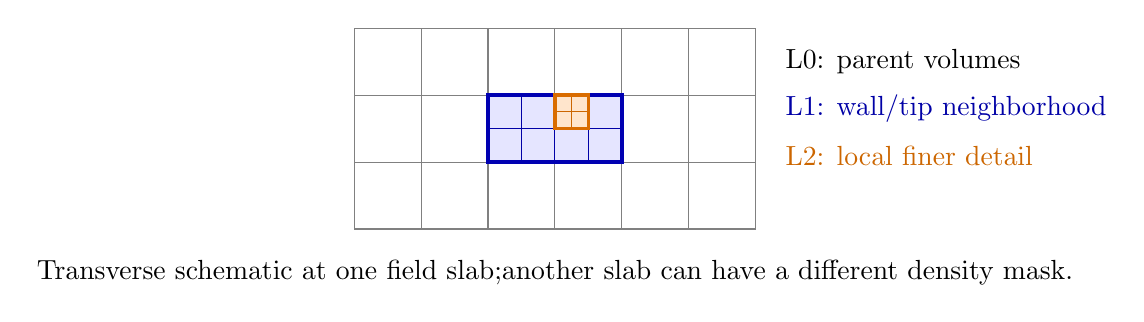
\begin{tikzpicture}[scale=.85]
\draw[step=1,gray] (0,0) grid (6,3);
\fill[blue!10] (2,1) rectangle (4,2);
\draw[step=.5,blue!65!black] (2,1) grid (4,2);
\fill[orange!20] (3,1.5) rectangle (3.5,2);
\draw[step=.25,orange!80!black] (3,1.5) grid (3.5,2);
\draw[very thick,blue!70!black] (2,1) rectangle (4,2);
\draw[very thick,orange!85!black] (3,1.5) rectangle (3.5,2);
\node[anchor=west] at (6.3,2.5) {L0: parent volumes};
\node[anchor=west,blue!65!black] at (6.3,1.8) {L1: wall/tip neighborhood};
\node[anchor=west,orange!80!black] at (6.3,1.1) {L2: local finer detail};
\node[align=center] at (3,-.65) {Transverse schematic at one field slab;\newline
another slab can have a different density mask.};
\end{tikzpicture}
\caption{Illustrative hierarchy only, not an image of a saved plasma solution.
The actual masks are output at each frame. Proper nesting and buffers are
computed from the detector, not prescribed by this sketch.}
\end{figure}

\subsection{Conservative restriction and prolongation}
Restriction preserves number and signed parallel momentum:
\begin{equation}
 N_P=\frac{\sum_cV_cN_c}{V_P},\qquad
 M_P=\frac{\sum_cV_cM_c}{V_P},\qquad V_P=\sum_cV_c.
\end{equation}
For prolongation, fit a local background amplitude $A$ using neighboring
parent differences and the existing reference basis $B$. Write child
density as a background-shaped part plus a residual and transverse slopes.
Logical child offsets are centred by volume weights, ensuring zero
volume-weighted slope correction. Bounds and a common positivity factor
limit the slopes without changing the parent average. The special
proportional-background branch avoids artificial cancellation residuals
when true child densities are many orders below a parent mean.

Parallel velocity is reconstructed separately. Its child slope correction
is centred using \emph{particle} weights $V_cN_c$, not merely volume,
so $\sum V_cN_cu_c=V_PM_P$. Applying a volume-centred velocity correction
would in general violate momentum conservation when density varies.
The optional seed marker follows the same particle-consistent transfer.
Remap verifies global particle, signed momentum and tracer invariants with
the original states retained until migration and transfer finish.

\subsection{Density residual, gradient and curvature criteria}
For a local $3\times3$ transverse stencil let
$n_0$ be its centre and
$n_{\rm norm}=\max(10^{-3}N_{\rm scale},\max n_{uv})$.
Raw first and second logical differences give
\begin{equation}
 G=\max(|D_xn|,|D_yn|)/n_{\rm norm},\quad
 C=\sqrt{D_{xx}^2+D_{yy}^2+2D_{xy}^2}/n_{\rm norm}.
\end{equation}
The normalization scale is strictly a detector scale; it is not inserted
into densities or the potential coefficient.

In represented-background mode, the local coefficient is
\begin{equation}
 A=\frac{\sum_{d=1}^4(B_d-B_0)(n_d-n_0)}
          {\sum_{d=1}^4(B_d-B_0)^2},
\end{equation}
with zero when the denominator vanishes. Apply the differences instead to
$R_{uv}=(n_{uv}-n_0)-A(B_{uv}-B_0)$. This removes only what the current
background-preserving reconstruction can already represent. It neither
evolves an unperturbed control nor subtracts one from the physical state.
Density walls, tips and branches can therefore request resolution while
a quiet represented altitude gradient need not refine an entire domain.

Refine/keep thresholds differ: release qualification uses
$G_{\rm on/off}=0.125/0.0625$ and $C_{\rm on/off}=0.02/0.01$.
Fine child indicators are also inspected before coarsening; a smooth parent
average must not hide canceling child detail. Prospective-parent information
loss is
\begin{equation}
 L=\max_c|N_c-N_c^{\rm prospective}|/n_{\rm norm},
\end{equation}
where the prospective values use the production conservative prolongation.
$L>0.005$ retains refinement. Marker-bearing regions can use the tighter
$\min(0.005,0.1A_{\rm declared})$ bound.

\subsection{Velocity, conductivity and weak-seed protection}
The velocity criterion uses the Hessian norm of the current E-cross-B
drift, scaled by maximum tag interval divided by local physical spacing.
It therefore detects a dynamically developing tip or curvature even before
deep depletion forms. Its keep threshold is half the refine threshold.
Second differences of all four integrated conductivity tensor components
provide an independent \emph{field-space} request, also with half-threshold
hysteresis. That request need not refine density along the whole tube.

If seed protection is enabled, an advected material marker identifies
the protected envelope. The required declared seed wavelength is sampled
by at least 32 cells and the vertical envelope by at least 8 cells. Tagged
developing structure can invoke an additional declared branch wavelength.
Any location still unresolved at the available finest level is counted.
An amplitude cannot be recovered after a coarse initial mesh has erased it;
protect the shortest relevant early mode from initialization. The late-time
qualification explicitly disables historical seed-marker reconstruction
and retains the existing developed checkpoint state.

\subsection{Buffers, physical-time hysteresis and proper nesting}
Structure requests receive a transverse root-cell buffer and promotion over
the current along-field slab. There is no unconditional whole-tube OR of
density requests. Three-level macro requests include required parents around
fine requests, including slab contacts and corners. A previously refined
cell can coarsen only after both its quiet duration and residence duration
exceed the configured physical quiet time, 60 s in the qualification.
Zero-hold simultaneous coarsening remains outside the qualified policy.

A check is triggered by the maximum tag interval or earlier when accumulated
transverse travel reaches half an internal-root scale. Consequently a
30 s maximum interval can yield actual regrids every few seconds. The
time-based hysteresis prevents those frequent checks from immediately
removing recently added resolution. Buffers cover stencil support and
anticipated motion; they are not a prescription to refine a fixed rectangle
around all depleted cells.

The retained legacy detector uses a same-time upper-quartile longitude
reference, depletion/gradient thresholds and a quiet-check count. Its
policy differs from the production structure criterion; changing between
them is a changed numerical case, not a performance-only optimization.

\subsection{Conservation and relation to general AMR frameworks}
The hierarchy follows the need for conservative transfer, proper nesting
and consistent interface flux emphasized by established AMR methods
\citep{BergerColella,Stone2020,Toth2012}. Here all levels use the same
accepted time step and the same summed physical interface flux. There is
no subcycled flux register. The prescribed magnetic field is not evolved,
so MHD constrained-transport or divergence-preserving magnetic prolongation
does not apply. Importing an MHD refinement mechanism without these
distinctions would not specify an ESF method.

\section{MPI ownership and hybrid kernel safety}
\subsection{Root-row partition and migration}
The partition planner balances the cumulative row estimate
\begin{equation}
 W_j=\frac1{N_\parallel}\sum_{i,k}(1+3r_{ijk})+
 w_{\rm canonical}N_{x,\rm internal},
\end{equation}
where $r$ is the density fine mask and $w_{\rm canonical}=0.5$ in the
qualified case. Whole-row cuts approximate equal prefix work, then
three-level cuts align to pairs. The estimate does not fully model
macro coarsening, molecular chemistry cost or ghost work. With only 80
physical L0 rows, 64 MPI ranks necessarily have coarse granularity.

O$^+$ halos extend six internal rows per side for three levels and three
for two levels; molecular response halos have their own narrower slab
width. At 13500 s, reconstruction of the exact partition from saved masks
gives 48 ranks owning one L0 row and 16 owning two. The largest molecular
owned-cell count is 1.6 times the mean; the largest O$^+$ activity count is
about 1.658 times its mean. The arithmetic mean of per-rank O$^+$
ghost/backing-owned ratios is 5.219. These are work/storage counts, not
exclusive timing percentages or a predicted speedup.

Molecular state keeps global backing but only owned/valid ghost values may
be read during evolution. On repartition, old/new slab intersections
transfer only changed ownership into separate receive buffers. Old owned
values remain valid until all sends and O$^+$ remapping finish. Identical
ownership is a byte-preserving no-op. Full molecular gathers are reserved
for output/checkpoints.

\subsection{What OpenMP parallelizes}
Independent cell kernels include molecular response refresh, current-stage
pressure-log preparation, final pressure/source normalization, stage
updates and macro-cell chemistry. Each active O$^+$ volume maps to disjoint
canonical reaction cells. Workers accumulate private reaction/charge
diagnostics, followed by reductions. A worker does not call MPI or abort
through the MPI failure path; invalid states are reported to the main
thread first.

Molecular face traversal is parallel by whole nonintersecting grid lines:
all $x$ lines in one $j$ row, all $y$ lines in one $i$ column, and one $(j,i)$ field line for a field sweep. The field-coordinate index stays innermost and contiguous in memory. A line retains serial face order. Two workers cannot write the same
cell during one axis sweep, and axis sweeps are separated by barriers.
Only scalar budget reductions change summation order. Blindly threading
individual faces would race on both neighboring cells.

AMR O$^+$ face blocks remain on the main thread. Their different-sized
contacts and lazy \code{ready}/child reconstruction caches require a
separate ownership strategy. Likewise canonical electron reconstruction
calls lazy sampling and is not blindly threaded. All MPI/PETSc calls stay
on the main thread under FUNNELED support. The executable verifies the
provided MPI thread level for multiple workers.

\subsection{Placement and resource accounting}
Each rank must have an allowed CPU domain large enough for all workers;
one-core binding cannot support four effective workers. Qualification
checks actual thread counts, inherited affinity and disjoint same-node
rank masks. Rank/worker count, active threads and Slurm reserved CPUs are
reported separately. A 32-by-2 comparison has the same 64 active threads as
64-by-1; a 64-by-4 comparison has256 active threads even when both fit the
same previously reserved256-CPU allocation. Neither should be mislabeled
as a fourfold same-resource algorithmic speedup.
